\section{Europäische Integration}
\begin{multicols}{2}
	Nach dem 2. Weltkrieg wurde die Weltwirtschaft unter Federführung der USA neu geordnet (Bretton-Woods-Konferenz, 1944). 
	\begin{itemize}
		\item Internationaler Währungsfond (IWF)
		\item Weltbank (World Bank)
	\end{itemize}
	Dies ist der Start für die Europäische Integration im Spannungsfeld
	\begin{itemize}
		\item zwischen \textbf{Vertiefung} (von der Zollunion hin zur Europäischen Verfassung)
		\item und \textbf{Erweiterung} (von den Gründerländern D, F, I, NL, B, L hin zur Osterweiterung).
	\end{itemize}
	Das Ziel hierbei ist, dass zukünftig von keinem europäischen Land ein globaler Krieg ausgehen soll.\\
	
	\vfill\null
	\columnbreak
	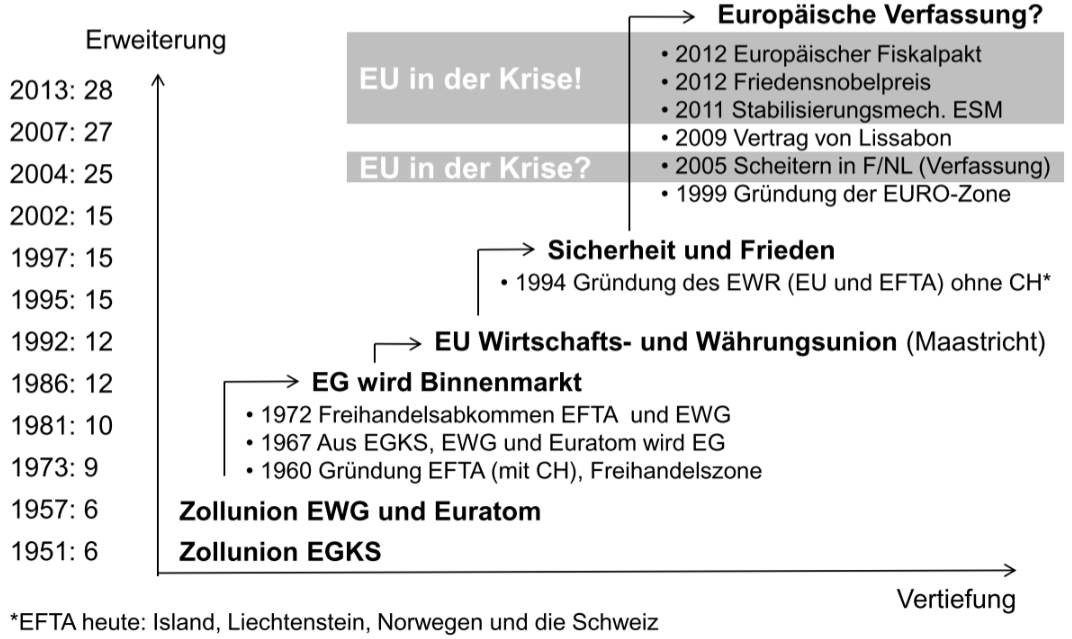
\includegraphics[width=\linewidth]{images/euintegration.png}
\end{multicols}

\subsection{Erweiterung der Europäischen Integration}
\begin{itemize}
	\item{\makebox[4cm]{1951 (EGKS der 6)\hfill}} Belgien, Deutschland, Frankreich, Italien, Luxemburg, Niederlande
	\item{\makebox[4cm]{1973 (EG der 9)\hfill}}  Dänemark, Irland, Vereinigtes Königreich
	\item{\makebox[4cm]{1981 (EG der 10)\hfill}} Griechenland
	\item{\makebox[4cm]{1986 (EG der 12)\hfill}} Portugal, Spanien
	\item{\makebox[4cm]{1995 (EU der 15)\hfill}} Finnland, Österreich, Schweden
	\item{\makebox[4cm]{2004 (EU der 25)\hfill}} Estland, Lettland, Litauen, Malta, Polen, Slowakei, Slowenien, Tschechien, Ungarn, Zypern
	\item{\makebox[4cm]{2007 (EU der 27)\hfill}} Bulgarien, Rumänien
	\item{\makebox[4cm]{2013 (EU der 28)\hfill}} Kroatien
	\item{\makebox[4cm]{2017 (EU der 27)\hfill}} Brexit (Vereinigtes Königsreich)
\end{itemize}

\subsubsection{EGKS (Zollunion), 1951}
\begin{itemize}
	\item EGKS: Europäische Gemeinschaft für Kohle und Stahl
	\item entstand unmittelbar nach WW2; europäischen Kontinent wirtschaftlich wieder aufbauen und dauerhafter Frieden
	\item Gründungsidee: französisch-deutsche Kohle- und Stahlproduktion zusammenführen
	\item nicht nur wirtschaftliche, sondern auch politische Logik, da diese Rohstoffe Grundlage der Industrie und Macht der beiden Länder
	\item politische Zielsetzung war, französisch-deutsche Solidarität zu stärken, das Gespenst des Krieges zu vertreiben und Weg für europäische Integration zu ebnen
	\item Laufzeit auf 50 Jahre begrenzt (2002 ausgelaufen)
	\item mit Blick auf späteren gemeinsamen Markt führt der Vertrag freien Warenverkehr ohne Zölle und Abgaben ein
	\item diskriminierende Praktiken, Subventionen und Beihilfen oder Sonderlasten sind untersagt
	\item Mitglieder gaben erstmals (begrenzt) nationale Souveränität zugunsten der Gemeinschaft ab
\end{itemize}

\subsubsection{EWG (Zollunion) und Euratom (Vertrag), 1957}
\begin{itemize}
	\item erste Anstrengung zur Integration stösst mit Scheitern der Europäischen Verteidigungsgemeinschaft EVG 1954 an Grenzen
	\item 1956 zwei Entwürfe für gemeinsamen europäischen Markt
	\begin{itemize}
		\item Schaffung eines allgemeinen gemeinsamen Marktes (EWG)
		\item Schaffung einer Europäischen Atomgeneinschaft (Euratom)
	\end{itemize}
	\item 1957 $"$Römische Verträge$"$ unterzeichnet
	\item zwei Ziele mit EWG
	\begin{enumerate}
		\item Umgestaltung der wirtschaftlichen Bedingungen des Handels und der Produktion auf Gebiet der Gemeinschaft
		\item politischeres Ziel: sieht EWG als Beitrag zur Errichtung eine politischen Europas und stellt Schritt in Richtung einer umfassenderen Integration dar
	\end{enumerate}
	\item beruht auf berühmten $"$vier Freiheiten$"$ zum freien Verkehr von
	\begin{enumerate}
		\item Waren, 
		\item Personen,
		\item Dienstleistungen und
		\item Kapital
	\end{enumerate}
	\item führt einheitlichen Wirtschaftsraum mit freiem Wettbewerb zwischen Unternehmen ein
	\item schafft Zölle und Einfuhrkontingente innerhalb der Zollunion ein $\rightarrow$ Aussengrenze für Waren aus Drittstaaten
	\item gemeinsame Handelspolitik auf Gemeinschafts- und nicht staatlicher Ebene $\rightarrow$ Unterschied zu reiner Freihandelszone
\end{itemize}

\subsubsection{EFTA (Freihandelszone)}
\begin{itemize}
	\item 1960 durch Stockholmer Konvention Europäische Freihandelsassoziation gegründet
	\item 7 Gründungsmitglieder: Schweiz, Dänemark, Grossbritannien, Norwegen, Österreich, Portugal, Schweden
	\item heutige Mitglieder: Schweiz, Norwegen, Island
	\item Grund: Nichtzustandekommen einer grossen Freihandelszone in Westeuropa und Gründung der EWG 1957
	\item Ziele:
	\begin{itemize}
		\item gemeinsames Auftreten der Mitgliedsstaaten ggü. der EWG, um wirtschaftliche Nachteile zu vermeiden
		\item um zu beweisen, dass eine Freihandelszone in Europa funktionieren könnte
	\end{itemize} 
\end{itemize}

\subsubsection{EU (Wirtschaftsunion), 1992}
\begin{itemize}
	\item Vor Inkrafttreten des Vertrags über die Europäische Union war die EWG der Kristallisationskern der Europäischen Integration (Grundlage zur Schaffung von Zollunion und Binnenmarkt)
	\item 1992 in Maastricht weiterentwickeltes rechtliches Regelungsgefüge ruht auf drei Säulen:
	\begin{enumerate}
		\item Die Europäische Gemeinschaft, die aus den EG-Gründungsverträgen von 1957 hervorgegangen ist und die in Maastricht weiter vertieft wurde, bleibt das tragende Element
		\item der Einstieg in eine $"$Gemeinsame Aussen- und Sicherheitspolitik$"$
		\item und in die $"$Zusammenarbeit der Justiz- und Innenminister$"$ erschloss neue, wichtige Handlungsbereiche.
	\end{enumerate}
	\item Vertrag über EU hat eine zentrale Botschaft:
	\begin{itemize}
		\item Die EU soll mehr sein als eine Wirtschaftsgemeinschaft. Die EU-Mitgliedsstaaten wollen die Politische Union Europas (EPU).
	\end{itemize}
 	\item Vertrag von Maastricht ist keine auf Dauer angelegte europäische $"$Verfassung$"$, die EU kein Staat im traditionellen Sinne $\rightarrow$ wird sich mit Vertragsänderungen zu einer Staatenverbindung ganz eigener Art weiterentwickeln
 	\item zwei bereits stattgefundene Revisionen in Amsterdam und Nizza
\end{itemize}

\subsubsection{EWU (Währungsunion), 1992}
\label{sec:EWU}
\begin{itemize}
	\item EWU stellt Zusammenschluss der EU-Mitgliedsstaaten auf Geld- und Währungspolitikgebiet dar
	\item seit Errichtung 1999 mit elf Staaten (Belgien, Deutschland, Finnland, Frankreich, Irland, Italien, Luxemburg, Niederlande, Österreich, Portugal, Spanien) traten acht weitere bei (2001-2015: Griechenland, Slowenien, Malta, Zypern, Slowakei, Estland, Lettland, Litauen)
	\item EU-Mitglieder die noch nicht den Euro eingeführt haben, sind grundsätzlich verpflichtet, der EWU beizutreten, sobald die festgelegten Konvergenzkriterien erfüllt werden
	\item Ausnahmen: Dänemark und Grossbritannien, die eine Sonderstellung aushandelten
	\item Konvergenzkriterien:
	\begin{description}
		\item[Preisstabilität:] Die Inflationsrate darf nicht mehr als 1,5 Prozentpunkte über derjenigen der drei preisstabilsten Mitgliedsländer der EU liegen.
		\item[Höhe der langfristigen Zinsen:] Die langfristigen Nominalzinssätze dürfen nicht mehr als zwei Prozentpunkte über den entsprechenden Zinssätzen der drei preisstabilsten Mitgliedsländer der EU liegen.
		\item[Haushaltsdiziplin:] Das jährliche öffentliche Defizit sollte grundsätzlich nicht mehr als 3\%, der öffentliche Schuldenstand nicht mehr als 60\% des BIP betragen.
		\item[Wechselkursstabilität:] Der Beitrittskandidat muss mindestens zwei Jahre am $"$Wechselkursmechanismus II$"$ teilgenommen haben. Dabei darf der Wechselkurs der eigenen Währung nicht starken Schwankungen ggü. dem Euro ausgesetzt gewesen sein.
	\end{description}
\end{itemize}
\clearpage

\subsubsection{EWR (Binnenmarkt zw. EU und EFTA), 1994}
\begin{itemize}
	\item 1992 unterzeichneten die damals zwölf EU-und EFTA-Mitglieder (Österreich, Finnland, Norwegen, Island, Schweden, Schweiz, Liechtenstein) den Vertrag zur Gründung des Europäischen Wirtschaftsraums EWR, trat 1994 in Kraft
	\item Schweiz entschied sich in einem Referendum gegen den Beitritt zum EWR $\rightarrow$ inzwischen durch $"$bilaterale Verträge$"$ mit EU dennoch den Status eines $"$quasi-EWR-Mitglieds$"$ erreicht \footnote{Wie lange noch?}
\end{itemize}

\subsection{Das Verhältnis der Schweiz zu Europa}
\begin{multicols}{2}
	Nach dem Nationalrat hat auch der Ständerat den Rückzug des Beitrittgesuchs von 1992 beschlossen: Ein historischer Entscheid ohne Folgen.\\
	Der Ständerat hat im Juni 2016 mit 27 zu 13 Stimmen und zwei Enthaltungen einer Motion von SVP-Nationalrat Lukas Reimann zugestimmt, die den Bundesrat auffordert, das EU-Beitrittsgesuch von 1992 zurückzuziehen. Der Nationalrat hatte bereits im März in diesem Sinne entschieden, mit 126 zu 46 Stimmen bei 18 Enthaltungen.\\
	Wie zieht man ein 24-jähriges Beitrittsgesuch zurück, das in einem Brüsseler Keller in einem Archiv lagert? Der Bundesrat werde der EU mitteilen, das Gesuch sei $"$als zurückgezogen zu betrachten$"$, sagte Aussenminister Didier Burkhalter.
	\vfill\null
	\columnbreak
	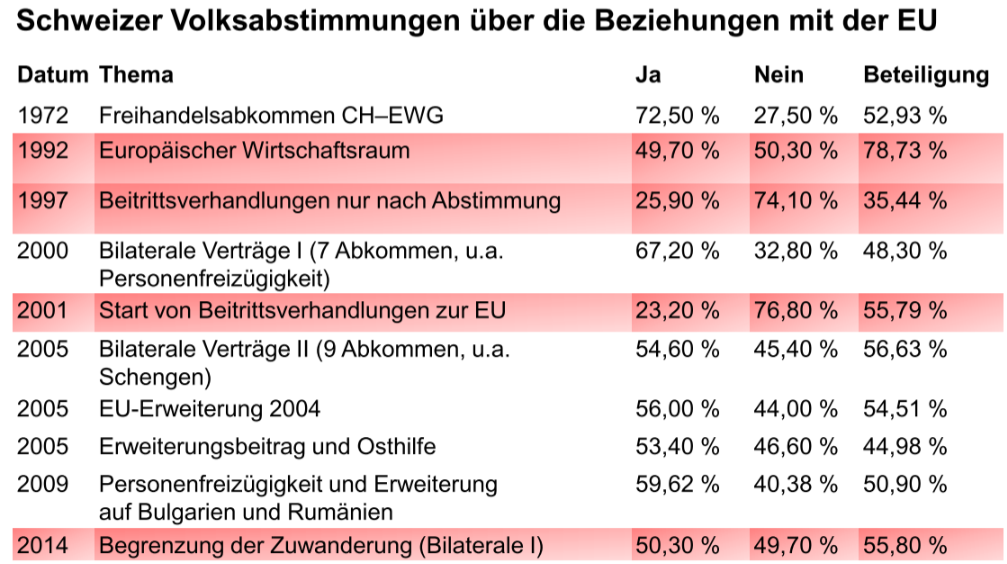
\includegraphics[width=\linewidth]{images/beziehung.png}
	2014 Begrenzung der Zuwanderung (Bilaterale I) $\rightarrow$ Kündigung der Bilaterale I
\end{multicols}
\clearpage
\pagebreak